\chapter{Financeiro dos meios de transporte}
\label{ch:identificador}
\section{Bairros e Faturamento}

\textbf{Bela Vista}
\begin{itemize}
    \item Raio: 2,6 km
    \item Comércios: 11.970
    \item Média: R\$ 143,64/ R\$ 12,00 / 2,6 km
    \item Semanal: R\$ 143,64 *7 = R\$ 1.005,48
    \item Mensal: R\$ 143,64 *30 = R\$ 4.309,2
\end{itemize} \\

\textbf{Bom Retiro}
\begin{itemize}
    \item Raio: 1.055 km
    \item Comércios: 10.036
    \item Média: R\$ 138,99/ R\$ 14,61/1,055 km
    \item Semanal: R\$ 138,99*7 = R\$ 972,93
    \item Mensal: R\$ 138,99*30 = R\$ 4.169,7
\end{itemize}\\

\textbf{Cambuci}
\begin{itemize}
    \item Raio: 3,9 km
    \item Comércios: 9.758
    \item Média: R\$ 258,58/ R\$ 26,50 / 3,9 km
    \item Semanal: R\$ 258,58*7 = R\$ 1.810,06
    \item Mensal: R\$ 258,58*30 = R\$ 7.757,4
\end{itemize}\\

\textbf{Consolação}
\begin{itemize}
    \item Raio: 85,9 km
    \item Comércios: 13.703
    \item Média: R\$ 16,210,64/1183,00 / 85,9 km
    \item Semanal: R\$ 16,210,64*7 = R\$ 113.474,48
    \item Mensal: R\$ 16,210,64*30 = R\$ 486.319,2
\end{itemize}\\ 

\textbf{Higienópolis}
\begin{itemize}
    \item Raio: 3,5 km
    \item Comércios: 7.979 Pontos:
    \item Média: R\$ 315,17/39,50 / 3,5 km ≈ R\$ 11,29 por km.
    \item Semanal: R\$ 315,17*7 = R\$ 2.206,19
    \item Mensal: R\$ 315,17*30 = R\$ 9.455,1
\end{itemize}\\

\textbf{Liberdade}
\begin{itemize}
    \item Raio: 3,7 km
    \item Comércios: 9.422
    \item Média: R\$ 396,66/42,10 / 3,7 km ≈ R\$ 11,378 por km
    \item Semanal: R\$ 396,66*7 = R\$ 2.776,62
    \item Mensal: R\$ 396,66*30 = R\$ 11.899,8
\end{itemize}\\

\textbf{República}
\begin{itemize}
    \item Raio: 2,3 km
    \item Comércios: 9.937
    \item Média: R\$ 244,45/R24,60 / 2,3 km ≈ R\$ 10,70 por km.
    \item Semanal: R\$ 244,45*7 = R\$ 1.711,15
    \item Mensal: R\$ 244,45*30 = R\$ 7.333,5
\end{itemize}\\

\textbf{Santa Cecília}
\begin{itemize}
    \item Raio: 2,1 km
    \item Comércios: 9.351
    \item Média: R\$ 93,51/10,00 / 2,1 km ≈ R\$ 4,76 por km.
    \item Semanal: R\$ 93,51 * 7 = R\$ 654,57
    \item Mensal: R\$ 93,51 * 30 = R\$ 2.805,3
\end{itemize}\\

\textbf{Sé}
\begin{itemize}
    \item Raio: 2,1 km
    \item Comércios: 4.473
    \item Média: R\$ 44,73/10,00 / 2,1 km ≈ R\$ 4,76/km.
    \item Semanal: R\$ 44,73 * 7 = R\$ 313,11
    \item Mensal = R\$ 44,73 * 30 = R\$ 1.341,90
\end{itemize}


\section{Despesas}

Meios de Transportes: será usado modelos de motociatas elétricas da montara indiana OLA e drones para entregas da empresa SPEEDBIRD além dos funcionários de todos os ramos atuando na companhia.

\section{Motocicleta Elétrica}

\begin{figure} [!ht]
    {\centering
    \caption{S1 Pro roxa}
    \includegraphics[height=0.3\linewidth]{figuras/S1 Pro.png}
    \label{fig:enter-label}
    \fonte{Ola Electric}
    }
\end{figure}

Aluguel será:
\begin{itemize}
    \item Diário: R\$ 20,00
    \item Semanal: R\$ 40,00
    \item Mensal: R\$ 100,00
\end{itemize}

Especificações: 
\begin{itemize}
    \item Espaço para bagageira - 34L.
    \item Velocidade máxima - 120 km/h.
    \item Alcance certificado de 195 km.
    \item Aceleração - 0 a 40 em 2,6 segundos.
    \item Liberte o poder de um motor de 11kW.
\end{itemize}

\begin{figure} [!ht]
   { \centering
    \caption{S1 Air verde}
    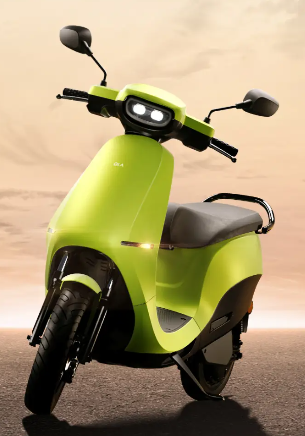
\includegraphics[height=0.3\linewidth]{figuras/S1 AIR.png}
    \label{fig:enter-label}
    \fonte{Ola Electric}
    }
\end{figure}

Aluguel será: 

\begin{itemize}
    \item Diário: R\$ 30,00
    \item Semanal: R\$ 50,00
    \item Mensal: R\$ 150,00
\end{itemize}

Especificações:

\begin{itemize}
    \item 151 KM de alcance.
    \item Espaço para bagageira de 34L
    \item Aceleração - 0-40 em 3,3 seg.
    \item Velocidade máxima de 90 km/h.\\\\\\\\\\\\\\\\\\
\end{itemize}

\begin{figure} [!ht]
    {\centering
    \caption{S1X vermelho}
    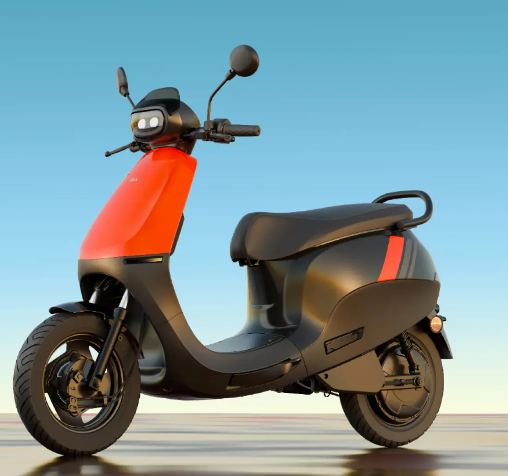
\includegraphics[height=0.2\linewidth]{figuras/S1X.png}
    \label{fig:enter-label}
    \fonte{Ola Electric}
    }
\end{figure}

Aluguel será: 
\begin{itemize}
    \item Diário: R\$ 50,00
    \item Semanal: R\$ 90,00
    \item Mensal: R\$ 350,00
\end{itemize}

Especificações:
\begin{itemize}
    \item 190 KM de alcance.
    \item Espaço para bagageira de 34L
    \item Aceleração: 0-40 em 3,3 seg.
    \item Velocidade máxima: 90 km/h.
\end{itemize}

Aplicativo Ola Electric controle sua scooter direto do seu telefone.

\begin{figure} [!ht]
    {\centering
    \caption{Aplicativo Ola Electric}
    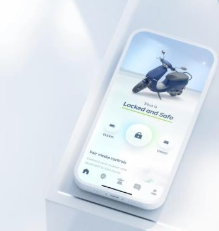
\includegraphics[height=0.4\linewidth]{figuras/app ola.png}
    \label{fig:enter-label}
    \fonte{Ola Electric}
    }
\end{figure}

Um mecânico de motos é de R\$ 1.512,00.
Um Entregador é de R\$ 1.706,00.

\section{Drones}

DLV-1 Possui uma capacidade de 2.5 kg de carga, podendo decolar com até 12.5 kg podendo percorrer 3 km de ida e volta.

\begin{figure}[!ht]
    \centering
    \caption{Drone DLV-1 Drop Flash.}
    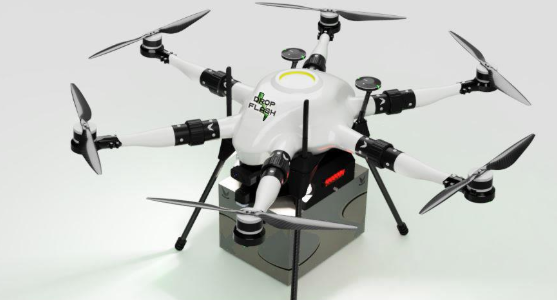
\includegraphics[width=0.6\textwidth]{figuras/DLV1.png}
    \label{fig:DLV1}\\
    \small Fonte: \url{https://www.speedbird.aero}
\end{figure}

Aluguel será: 
\begin{itemize}
    \item Diário: R\$ 100,00
    \item Semanal: R\$ 200,00
    \item Mensal: R\$ 500,00
\end{itemize}

Possui uma capacidade de 6 kg de carga e pode decolar com 25 kg de carga com 8 km de ida e volta.

\begin{figure}[!ht]
    \centering
    \caption{Drone DLV-2 Drop Flash.}
    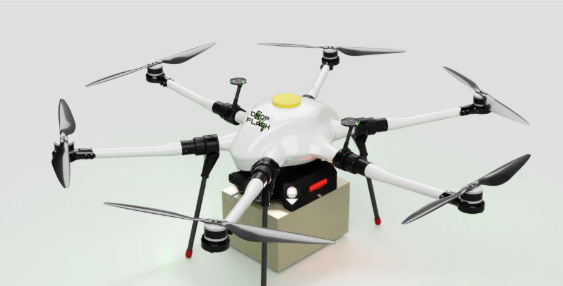
\includegraphics[width=0.6\textwidth]{figuras/Dlv 2.png}
    \label{fig:DLV2}\\
    \small Fonte: \url{https://www.speedbird.aero}
\end{figure}

Aluguel será: 
\begin{itemize}
    \item Diário: R\$ 200,00
    \item Semanal: R\$ 500,00
    \item Mensal: R\$ 1000,00
\end{itemize}

DLV-4 Possui uma capacidade de carga de até 5 kg, com peso máximo de decolagem de 25 kg, porém o diferencial do DLV-4 é a distância que pode percorrer, que é de até 40 km de ida e volta.

\begin{figure} [!ht]
   { \centering
    \caption{Drone DLV-4 Drop Flash.}
    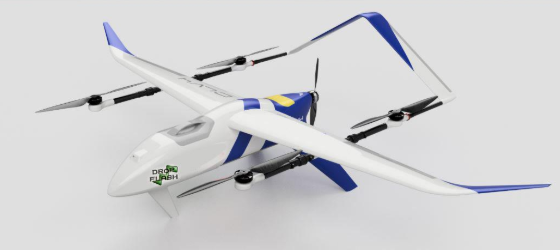
\includegraphics[width=0.6\linewidth]{figuras/dlv 4.png}
    \label{fig:enter-label}
    \fonte{https://www.speedbird.aero}
    }
\end{figure}

Aluguel será: 

\begin{itemize}
    \item Diário: R\$ 500,00
    \item Semanal: R\$ 1000,00
    \item Mensal: R\$ 3000,00
\end{itemize}

\section{Geral}

Pontos de decolagem e pouso Para cada região cadastrada existirá uma base para pouso, decolagem e manutenção dos drones. No total serão 9 bases e cada base terá 20 DLV-1, 20 DLV-2 e 10 DLV-4.

\begin{figure} [!ht]
    \centering
    \caption{Ilustração de um ponto de pouso e decolagem de drones da Drop Flash.}
    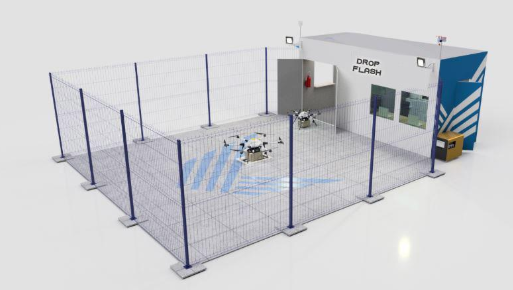
\includegraphics[width=0.4\linewidth]{figuras/p dec e po.png}
    \label{fig:enter-label}
    \fonte{https://www.speedbird.aero}
\end{figure}

Investimento total no drones será de 500 mil. Além doas aluguéis dos terraços dos prédios que media fica em R\$ 5.000,00 mais a parte de instalação e gasto com a rede elétrica variando dependo do lugar. Na parte dos salários um piloto de drone de carga habilitado é em média de R\$ 21.047,00.

\section{Programas}
O Cloud Control Station (CCS) do Speedbird é um poderoso conjunto de software projetado para fornecer infraestrutura tecnológica ponta a ponta para controle e monitoramento de aeronaves, proporcionando uma experiência de usuário segura e contínua. Os operadores podem planejar e definir corredores aéreos e rotas predefinidas para conectar droneportos estrategicamente localizados em cidades, hospitais, armazéns e centros de distribuição.

\begin{figure}[!ht]
  {  \centering
    \caption{Monitoramento das aeronaves}
    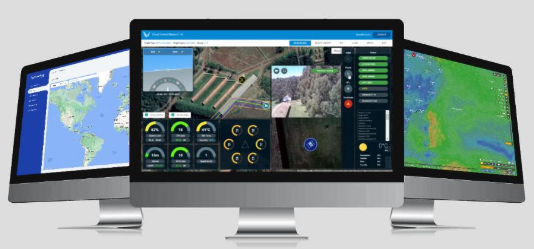
\includegraphics[width=0.5\linewidth]{programa.png}
    \label{fig:enter-label}
    \fonte{https://www.speedbird.aero}
    }
\end{figure}

Na parte dos Softwares de drones e motos será de R\$ 7.000,00 contando peças, internet 4G e 5G e atualizações dos mesmos